%  Data note: OBSCURA-Open-25. MDPI LaTeX template (official, downloaded from mdpi.com).
%  Journal is not yet chosen, so the generic option "notspecified" is used.
\documentclass[notspecified,datadescriptor,submit,oneauthor]{Definitions/mdpi}

\firstpage{1}
\makeatletter
\setcounter{page}{\@firstpage}
\makeatother
\pubvolume{1}
\issuenum{1}
\articlenumber{0}
\pubyear{2026}
\copyrightyear{2026}
\history{Received: date; Accepted: date; Published: date}

\Title{OBSCURA-Open-25: An Open Multi-Target Satellite Dataset and Facility-Grouped Validation Guidelines for Industrial Emission Sites}

\Author{Zulqarnain Ali $^{1}$}
\AuthorNames{Zulqarnain Ali}
\address{%
$^{1}$ \quad Affiliation to be added; ORCID 0009-0009-0281-882X}
\corres{Correspondence: zulqar445ali@gmail.com}

\abstract{Satellites measure methane and related combustion gases above industrial sites, but few open datasets pair facility-scale imagery with several gas measurements, and models trained on them are usually validated with random splits. We present OBSCURA-Open-25: 1355 samples from 25 industrial facilities in 15 countries, each pairing a 14-layer Sentinel-2 image chip with Sentinel-5P methane, nitrogen dioxide and carbon monoxide enhancements, an aerosol index and a fire intensity, plus weather, terrain and spectral features and a record of all 1825 attempted observation windows. We also give usage guidelines and a Python package (obscura\_open25) with a facility-grouped validation protocol. In a case study on the released files, a random split understates the error for unseen facilities by 11\% to 38\%, and for fire it reverses the conclusion: the model beats a zero prediction under a random split (0.64 against 0.91) and loses to it under a grouped split (1.04). Only the aerosol index is clearly predictable for new facilities. Re-running the collection reproduced 15 of 15 sampled windows exactly. The data are released under CC BY 4.0.}

\keyword{Earth observation; Sentinel-2; Sentinel-5P; methane; industrial emissions; cross-validation; spatial leakage; open data}

\begin{document}

\section{Summary}

Sentinel-5P measures methane over the whole globe almost daily \cite{veefkind}, but a single facility changes the column by little compared with retrieval noise, and cloud or quality filters often remove the reading altogether. Nitrogen dioxide, carbon monoxide and aerosols come from the same burning and venting. Earlier open resources pair Sentinel-2 with Sentinel-5P for ground-level nitrogen dioxide \cite{scheibenreif} or label methane plumes at known super-emitters \cite{vaughan}. We know of none that offers facility-level chips with several gas targets and a record of every attempted observation.

This note contributes three things: the dataset, guidelines for using it, and a measured example of why the guidelines matter. The example is a validation protocol that holds out whole facilities, because rows from one facility resemble each other \cite{roberts}. All numbers below are computed from the files of the Zenodo record (doi:10.5281/zenodo.23450639) with the code at \url{https://github.com/zulqarnainalipk/obscura-open-25}; \texttt{examples/reproduce\_note.py} repeats them. The 25 facilities are a subset of a larger collection built for a public machine learning competition, whose remaining facilities will be released, with a separate descriptor, after it ends.

\section{Data Description}

\textbf{Facilities and windows.} The facilities are refineries, gas plants, LNG terminals, oilfields, chemical sites, mines and a smelter in eight world regions (Figure~\ref{fig1}a). They were chosen for data quality: many samples, high gas availability, little cloud and all seasons covered. Each centre and image box (1.5 to 7.75 km) was checked by hand. Every second 5-day window from 1 January 2022 to 27 December 2023 was tried (1825). A window gives a sample if the least cloudy Sentinel-2 scene has at most 30\% cloud and at least one gas target exists: 1355 samples (74\%). A further 441 windows were too cloudy, 11 had no scene and 18 failed other checks. All attempts are listed.

\begin{figure}[H]
\centering
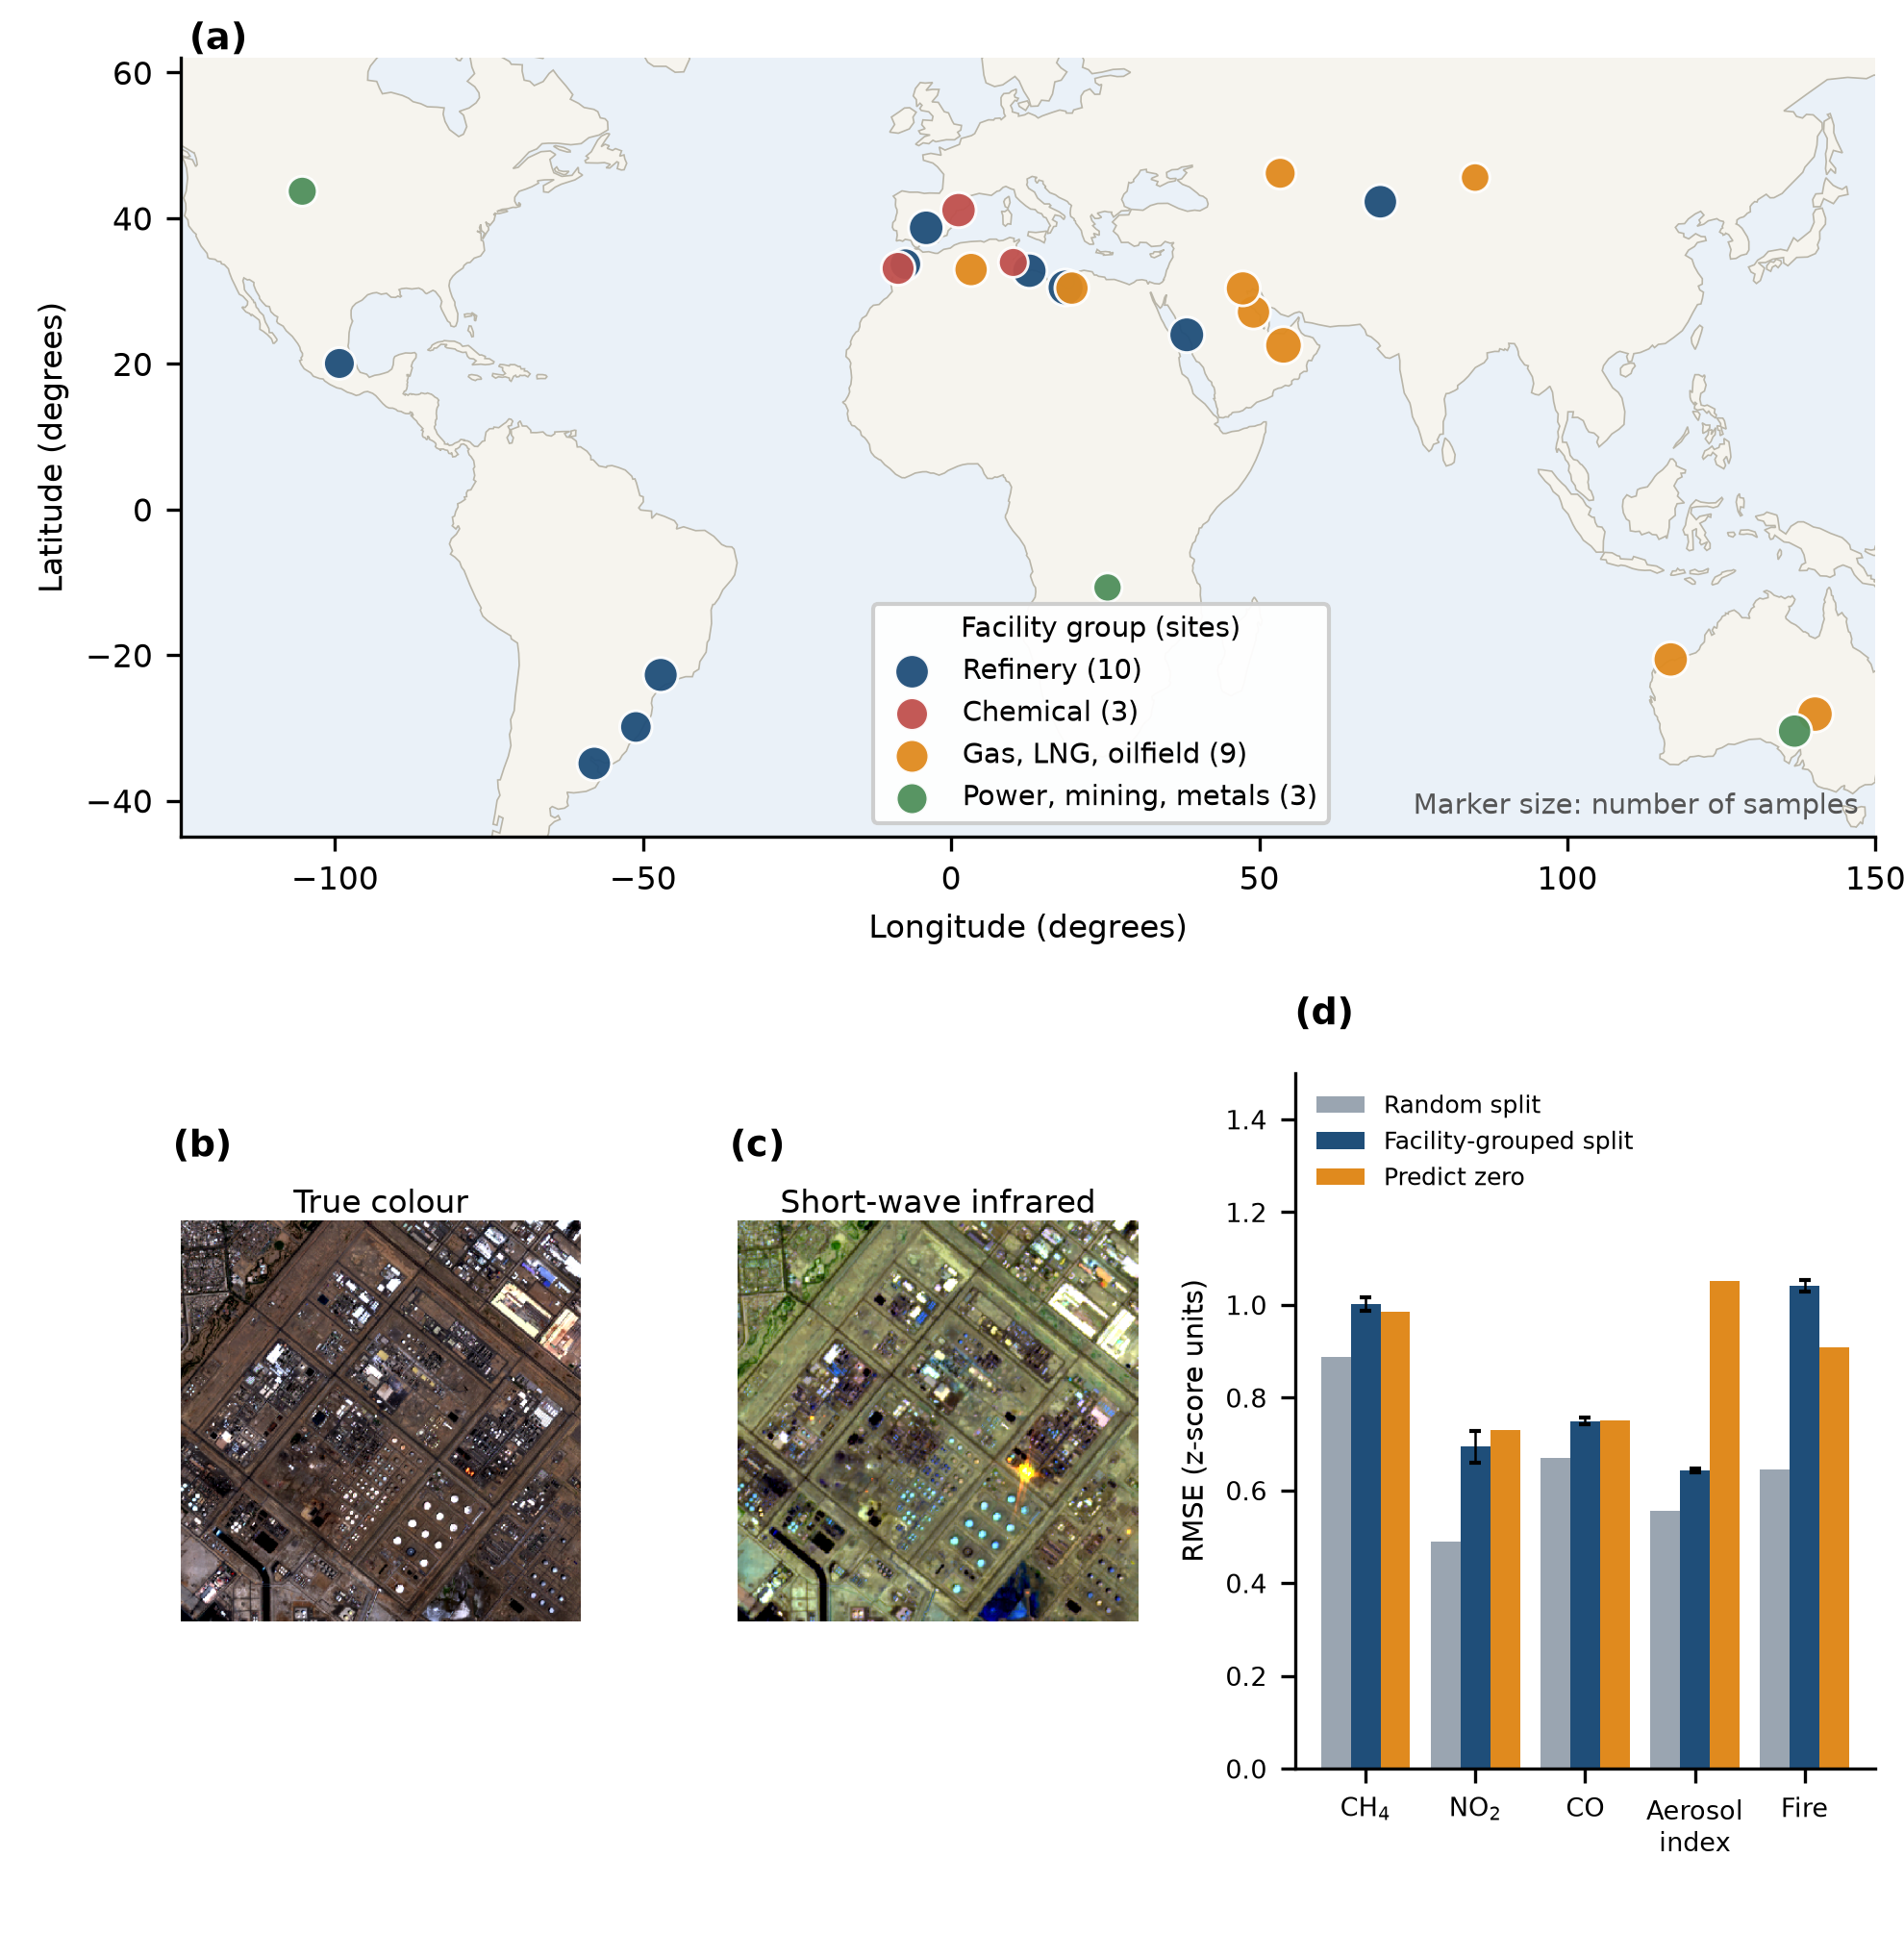
\includegraphics[width=\textwidth]{fig1.png}
\caption{OBSCURA-Open-25. (\textbf{a}) The 25 facilities by group; marker size shows the number of samples. (\textbf{b}) True-colour chip of one sample (Yanbu complex, Saudi Arabia, 20 March 2023; side 6 km). (\textbf{c}) The same chip in short-wave infrared (B12, B11, B4), where a flare glows orange. (\textbf{d}) The five targets of this sample, in physical units and as z-scores.\label{fig1}}
\end{figure}

\textbf{Chips.} Each chip is a $384\times384$ GeoTIFF with 14 layers: 12 Sentinel-2 Level-2A reflectance bands \cite{drusch}, the scene classification and the cloud probability. Pixels are 3.9 to 20.2 m, chips are not cloud-masked, and the grid carries a random offset below about 60 m.

\textbf{Targets.} Gas targets are Sentinel-5P methane, nitrogen dioxide and carbon monoxide \cite{veefkind}, read through Google Earth Engine \cite{gorelick}. Each is the mean over a 10 km window minus the median of a land-only ring from 30 to 75 km \cite{carroll}, excluding areas near other facilities, and is paired with the Sentinel-2 scene within one day. The aerosol index is the window mean. Fire intensity is the hottest NASA FIRMS anomaly \cite{giglio}, or zero. Methane exists for 49\% of samples, the other gases for 99\%. A blank means not measured, not zero. Values come in physical units and as z-scores.

\textbf{Features.} The 29 features are month, ERA5-Land weather \cite{munoz}, elevation and slope \cite{dem}, chip cloud share and 18 spectral indices.

\section{Data Records and Usage Guidelines}

The record has 40 files (2.2 GB) under CC BY 4.0: tables of facilities, samples, features and attempted windows, 25 chip archives (one per facility), documentation and checksums. Source scene identifiers are given for every sample. Four rules apply.

\begin{enumerate}[labelsep=2mm]
\item Read \texttt{sample\_id} as text; four identifiers look like numbers.
\item Fit and score each target only where it exists.
\item Validate by facility, never by row.
\item Remember that the sites are cleaner than typical ones and that chips are positioned to about 100 m.
\end{enumerate}

A minimal workflow:
{\footnotesize
\begin{verbatim}
from obscura_open25 import Dataset, compare_splits
ds = Dataset("data")           # 25 sites, 1355 samples
chip = ds.read_chip(ds.samples.sample_id.iloc[0])   # (14, 384, 384)
print(compare_splits(ds).round(3))
\end{verbatim}}

\section{Case Study: Random Versus Facility-Grouped Validation}

For each target, a gradient-boosted model on the 29 features was scored by five-fold cross-validation, once with random rows and once with whole facilities held out (five fold assignments each). Error is the RMSE in z-score units over measured samples; predicting zero is the reference (Table~\ref{tab1}).

\begin{table}[H]\centering
\caption{RMSE (z-score units). Lower is better.\label{tab1}}
\begin{tabular}{lcccc}
\toprule
\textbf{Target} & \textbf{Random} & \textbf{Grouped} & \textbf{Predict Zero} & \textbf{Understated By}\\
\midrule
Methane & 0.89 & 1.00 & 0.98 & 11\%\\
Nitrogen dioxide & 0.49 & 0.69 & 0.73 & 30\%\\
Carbon monoxide & 0.67 & 0.75 & 0.75 & 11\%\\
Aerosol index & 0.56 & 0.64 & 1.05 & 13\%\\
Fire & 0.64 & 1.04 & 0.91 & 38\%\\
\bottomrule
\end{tabular}
\end{table}

Every target looks better under a random split, probably because the model recognises a facility from its terrain and chip statistics and recalls its usual values (we did not test this directly). For fire the conclusion flips: a random split says the model beats a zero prediction, a grouped split says it does not. For unseen facilities only the aerosol index is clearly predictable, nitrogen dioxide is marginal, and methane and carbon monoxide show no gain. The spread over fold assignments was at most 0.034.

We also asked whether a methane reading can be predicted to exist, using grouped folds. The area under the ROC curve was 0.63 from weather, 0.58 from chip statistics and 0.70 from all features, so missing methane is only weakly predictable and mostly site-specific. This is why the attempted-window table is provided.

\section{Technical Validation}

All files match their checksums and 1355 chips exist for 1355 samples. In all chips the facility centre lies inside the chip, and the chip centre is a median of 48 m (at most 84 m) from it. Fifteen samples at 15 facilities, some with blank targets, were rebuilt from the public archives with the documented procedure: all were identical in every field and pixel. This was a re-run of the same procedure, not an independent implementation. Fourteen consistency checks on value limits, dates, pixel counts and reasons for blanks passed. The satellite products were not compared with ground measurements, and small enhancements of either sign are mostly noise.

\vspace{6pt}

\authorcontributions{Conceptualization, methodology, software, validation, formal analysis, investigation, data curation, writing (original draft and review), and visualization: Z.A. The author has read and agreed to the published version of the manuscript.}

\funding{This research received no external funding.}

\section*{Data Availability Statement}
The dataset is at Zenodo (\url{https://doi.org/10.5281/zenodo.23450639}, CC BY 4.0). The code is at \url{https://github.com/zulqarnainalipk/obscura-open-25} (MIT).

\acknowledgments{Contains modified Copernicus Sentinel data (2022--2023) and modified Copernicus Climate Change Service information. Fire data are from NASA FIRMS. The author used the AI assistant Claude (Anthropic) for programming help and drafting, checked the data and text, and is responsible for the content.}

\conflictsofinterest{The author declares no conflict of interest.}

\reftitle{References}

\begin{thebibliography}{999}
\bibitem[Veefkind et~al.(2012)]{veefkind}
Veefkind, J.P.; Aben, I.; McMullan, K.; F{\"o}rster, H.; de~Vries, J.; Otter, G.; Claas, J.; Eskes, H.J.; de~Haan, J.F.; Kleipool, Q.; et~al. TROPOMI on the ESA Sentinel-5 Precursor: A GMES Mission for Global Observations of the Atmospheric Composition for Climate, Air Quality and Ozone Layer Applications. {\em Remote Sens. Environ.} {\bf 2012}, {\em 120}, 70--83. doi:10.1016/j.rse.2011.09.027.
\bibitem[Scheibenreif et~al.(2022)]{scheibenreif}
Scheibenreif, L.; Mommert, M.; Borth, D. Toward Global Estimation of Ground-Level NO$_2$ Pollution With Deep Learning and Remote Sensing. {\em IEEE Trans. Geosci. Remote Sens.} {\bf 2022}, {\em 60}, 4705914. doi:10.1109/TGRS.2022.3160827.
\bibitem[Vaughan et~al.(2024)]{vaughan}
Vaughan, A.; Mateo-Garc{\'\i}a, G.; G{\'o}mez-Chova, L.; R{\r{u}}{\v{z}}i{\v{c}}ka, V.; Guanter, L.; Irakulis-Loitxate, I. CH4Net: A Deep Learning Model for Monitoring Methane Super-Emitters with Sentinel-2 Imagery. {\em Atmos. Meas. Tech.} {\bf 2024}, {\em 17}, 2583--2593. doi:10.5194/amt-17-2583-2024.
\bibitem[Drusch et~al.(2012)]{drusch}
Drusch, M.; Del~Bello, U.; Carlier, S.; Colin, O.; Fernandez, V.; Gascon, F.; Hoersch, B.; Isola, C.; Laberinti, P.; Martimort, P.; et~al. Sentinel-2: ESA's Optical High-Resolution Mission for GMES Operational Services. {\em Remote Sens. Environ.} {\bf 2012}, {\em 120}, 25--36. doi:10.1016/j.rse.2011.11.026.
\bibitem[Giglio et~al.(2016)]{giglio}
Giglio, L.; Schroeder, W.; Justice, C.O. The Collection 6 MODIS Active Fire Detection Algorithm and Fire Products. {\em Remote Sens. Environ.} {\bf 2016}, {\em 178}, 31--41. doi:10.1016/j.rse.2016.02.054.
\bibitem[Gorelick et~al.(2017)]{gorelick}
Gorelick, N.; Hancher, M.; Dixon, M.; Ilyushchenko, S.; Thau, D.; Moore, R. Google Earth Engine: Planetary-Scale Geospatial Analysis for Everyone. {\em Remote Sens. Environ.} {\bf 2017}, {\em 202}, 18--27. doi:10.1016/j.rse.2017.06.031.
\bibitem[Carroll et~al.(2009)]{carroll}
Carroll, M.L.; Townshend, J.R.; DiMiceli, C.M.; Noojipady, P.; Sohlberg, R.A. A New Global Raster Water Mask at 250 m Resolution. {\em Int. J. Digit. Earth} {\bf 2009}, {\em 2}, 291--308. doi:10.1080/17538940902951401.
\bibitem[Mu{\~n}oz-Sabater et~al.(2021)]{munoz}
Mu{\~n}oz-Sabater, J.; Dutra, E.; Agust{\'\i}-Panareda, A.; Albergel, C.; Arduini, G.; Balsamo, G.; Boussetta, S.; Choulga, M.; Harrigan, S.; Hersbach, H.; et~al. ERA5-Land: A State-of-the-Art Global Reanalysis Dataset for Land Applications. {\em Earth Syst. Sci. Data} {\bf 2021}, {\em 13}, 4349--4383. doi:10.5194/essd-13-4349-2021.
\bibitem[European Space Agency and Airbus(2022)]{dem}
European Space Agency; Airbus. Copernicus Global Digital Elevation Model. 2022. doi:10.5270/ESA-c5d3d65.
\bibitem[Roberts et~al.(2017)]{roberts}
Roberts, D.R.; Bahn, V.; Ciuti, S.; Boyce, M.S.; Elith, J.; Guillera-Arroita, G.; Hauenstein, S.; Lahoz-Monfort, J.J.; Schr{\"o}der, B.; Thuiller, W.; et~al. Cross-Validation Strategies for Data with Temporal, Spatial, Hierarchical, or Phylogenetic Structure. {\em Ecography} {\bf 2017}, {\em 40}, 913--929. doi:10.1111/ecog.02881.
\end{thebibliography}

\end{document}
